\subsubsection{Hochregallager System}
Die Partnerfirma des Projekts entwickelt und produziert klassische automatische Hochregallager. \textit{Warum also nicht deren Produkte verwenden?}

\paragraph{Ein Fahrradturm mit LTW Produkten wird vom Projektteam folgend skizziert:}
Im EG gibt es die Einlagerungsplätze. Jeder dieser Plätze hat von vorne mit Rolltoren verschließbare Öffnungen, an welche die Boxen rückseitig geschoben werden. Das System erkennt nach ein paar Tagen automatisch die Hauptnutzungszeiten, und weiß, wann aus oder eingelagert wird. Nach diesen Erfahrungswerten wird eine unterschiedliche Anzahl an leeren Fahrradboxen und Paketboxen bereitgehalten. Ebenfalls besteht die Möglichkeit, dass die App dem Turm meldet, wenn sich jemand dem Turm nähert und dann dessen Box schon im vorherein in einen freien Platz gestellt wird. Kommt es dann zur Auslagerung muss nur noch das Rolltor und die Boxentüre geöffnet werden und das \ac{RBG} kann im Hintergrund andere Aufgaben erledigen.

\noindent Um nach einem Vorgang prüfen zu können, ob die Box wieder leer ist, kommen Höhensensoren, Wärmebildkameras und Bewegungsmelder zum Einsatz. Ist der Platz wirklich menschenleer, wird die Box von hinten vom Regalbediengerät aufgenommen. Dahinter ist der Schacht, durch den die Boxen verfahren werden. In den in beliebiger Anzahl vorhandenen Stöcken finden sich die Lagerplätze. Je nach Ausführung wird hier beidseitig oder einseitig gelagert.

\noindent Das \ac{RBG} verfährt nur in horizontaler und gleichzeitig in vertikaler Richtung zu einem freien Platz. Dort angekommen wird die Box in das Regal übergeschoben.

\begin{figure}[H]
    \centering
    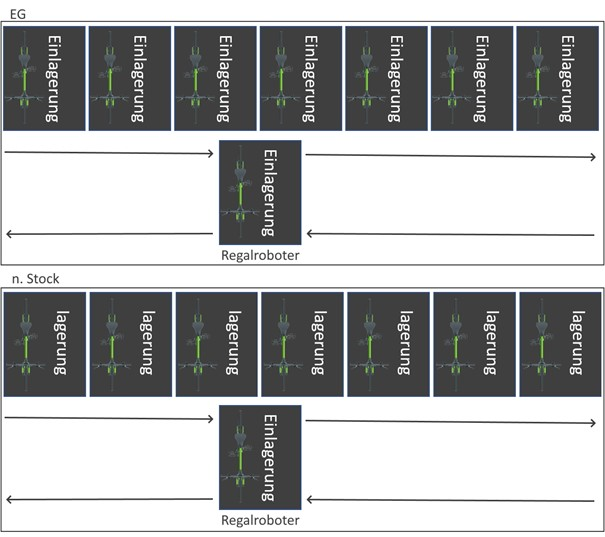
\includegraphics[width=0.5\textwidth]{images/hochregallager2d.jpg}
    \caption{Hochregallager 2D Ansicht}
    \label{fig:hochregallager2d}
\end{figure}

\clearpage

Je nach den lokalen Anforderungen kann das Konzept variieren. Mehrere Einlagerungsplätze einzubauen ist dabei am billigsten. Reicht auch das nicht aus, kann die Anzahl der \ac{RBG} erhöht werden, es gibt Systeme, allerdings in Lagern, bei denen mehrere Roboter gleichzeitig im Gebäude in Betrieb sind.

\indent Reicht der die Lageranzahl nicht aus, besteht im Gegensatz zum Rondell, neben der Möglichkeit höher zu bauen, auch die Variante die Grundfläche zu erhöhen. Zieht man die Gebäudegeometrie so in die Länge, erhöht sich die Anzahl an Stellplätzen proportional um den doppelten Faktor der übereinander angeordneten Boxen.

\begin{figure}[H]
    \centering
    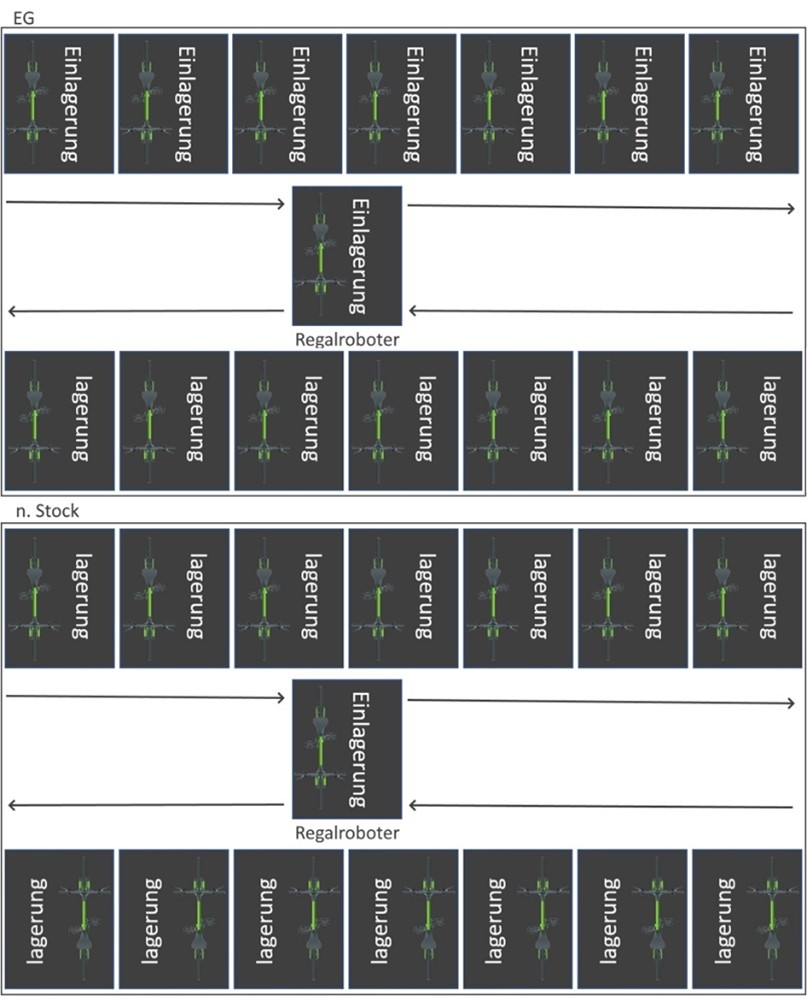
\includegraphics[width=0.4\textwidth]{images/hochregallager2ddoppelt.jpg}
    \caption{Hochregallager mit doppelten Plätzen, 2D Ansicht}
    \label{fig:hochregallager2ddoppelt}
\end{figure}

\begin{figure}[H]
    \centering
    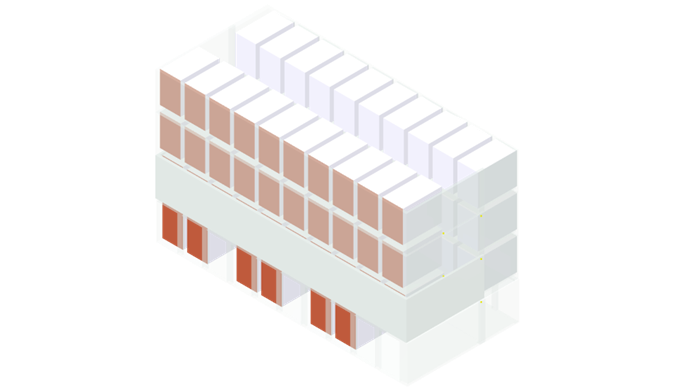
\includegraphics[width=0.6\textwidth]{images/hochregallager3d.png}
    \caption{Hochregallager 3D Ansicht}
    \label{fig:hochregallager3d}
\end{figure}

